%% 
%% Copyright 2007-2024 Elsevier Ltd
%% 
%% This file is part of the 'Elsarticle Bundle'.
%% ---------------------------------------------
%% 
%% It may be distributed under the conditions of the LaTeX Project Public
%% License, either version 1.3 of this license or (at your option) any
%% later version.  The latest version of this license is in
%%    http://www.latex-project.org/lppl.txt
%% and version 1.3 or later is part of all distributions of LaTeX
%% version 1999/12/01 or later.
%% 
%% The list of all files belonging to the 'Elsarticle Bundle' is
%% given in the file `manifest.txt'.
%% 
%% Template article for Elsevier's document class `elsarticle'
%% with harvard style bibliographic references

\documentclass[preprint,12pt,authoryear]{elsarticle}

%% Use the option review to obtain double line spacing
%% \documentclass[authoryear,preprint,review,12pt]{elsarticle}

%% Use the options 1p,twocolumn; 3p; 3p,twocolumn; 5p; or 5p,twocolumn
%% for a journal layout:
%% \documentclass[final,1p,times,authoryear]{elsarticle}
%% \documentclass[final,1p,times,twocolumn,authoryear]{elsarticle}
%% \documentclass[final,3p,times,authoryear]{elsarticle}
%% \documentclass[final,3p,times,twocolumn,authoryear]{elsarticle}
%% \documentclass[final,5p,times,authoryear]{elsarticle}
%% \documentclass[final,5p,times,twocolumn,authoryear]{elsarticle}

%% For including figures, graphicx.sty has been loaded in
%% elsarticle.cls. If you prefer to use the old commands
%% please give \usepackage{epsfig}

%% The amssymb package provides various useful mathematical symbols
\usepackage{amssymb}
%% The amsmath package provides various useful equation environments.
\usepackage{amsmath}
%% The amsthm package provides extended theorem environments
%% \usepackage{amsthm}
\usepackage{url}
\usepackage{graphicx}
\usepackage{lineno} 

%% The lineno packages adds line numbers. Start line numbering with
%% \begin{linenumbers}, end it with \end{linenumbers}. Or switch it on
%% for the whole article with \linenumbers.
%% \usepackage{lineno}

\journal{Climate Services}

\begin{document}

\begin{frontmatter}

%% Title, authors and addresses

%% use the tnoteref command within \title for footnotes;
%% use the tnotetext command for theassociated footnote;
%% use the fnref command within \author or \affiliation for footnotes;
%% use the fntext command for theassociated footnote;
%% use the corref command within \author for corresponding author footnotes;
%% use the cortext command for theassociated footnote;
%% use the ead command for the email address,
%% and the form \ead[url] for the home page:
%% \title{Title\tnoteref{label1}}
%% \tnotetext[label1]{}
%% \author{Name\corref{cor1}\fnref{label2}}
%% \ead{email address}
%% \ead[url]{home page}
%% \fntext[label2]{}
%% \cortext[cor1]{}
%% \affiliation{organization={},
%%            addressline={}, 
%%            city={},
%%            postcode={}, 
%%            state={},
%%            country={}}
%% \fntext[label3]{}

\title{Balancing Accuracy versus Precision: Enhancing the Usability of Sub-Seasonal Forecasts} %% Article title

%% use optional labels to link authors explicitly to addresses:
%% \author[label1,label2]{}
%% \affiliation[label1]{organization={},
%%             addressline={},
%%             city={},
%%             postcode={},
%%             state={},
%%             country={}}
%%
%% \affiliation[label2]{organization={},
%%             addressline={},
%%             city={},
%%             postcode={},
%%             state={},
%%             country={}}


\author[label1,label2]{Etienne Dunn-Sigouin} %% Author name
\ead{etdu@norceresearch.no}


\author[label1,label2]{Erik W. Kolstad}


\author[label1,label2]{C. Ole Wulff}

\author[label1,label2,label3,label4]{Douglas J. Parker}

\author[label3,label5]{Richard J. Keane}


%% Author affiliation
\affiliation[label1]{organization={NORCE Norwegian Research Center AS},%Department and Organization 
            city={Bergen},
            country={Norway}}

\affiliation[label2]{organization={Bjerknes Center for Climate Research},%Department and Organization 
            city={Bergen},
            country={Norway}}

\affiliation[label3]{organization={School of Earth and Environment, University of Leeds},%Department and Organization 
            city={Leeds},
            country={UK}}

\affiliation[label4]{organization={NCAS National Centre for Atmospheric Science, University of Leeds},%Department and Organization 
            city={Leeds},
            country={UK}}

\affiliation[label5]{organization={Met Office},%Department and Organization 
            city={Exeter},
            country={UK}}
            
%% Abstract
\begin{abstract}
%% Text of abstract
Forecasts are essential for climate adaptation and preparedness, such as in early warning systems and impact models. A key limitation to their practical use is often their coarse spatial grid spacing. However, another less frequently discussed but crucial limitation is that forecasts are often more precise than they are accurate when their grid spacing is finer than the scales they can accurately predict. Here, we adapt the fractions skill score, a metric conventionally used to quantify spatial forecast accuracy by the meteorological community, to help users navigate the trade-off between forecast accuracy versus precision. We demonstrate how this trade-off can be visualized for daily European precipitation, focusing on deterministic predictions of anomalies and probabilistic predictions of extremes, derived from three years of sub-seasonal forecasts from the European Centre for Medium-Range Weather Forecasts (ECMWF). Our results show that decreasing precision through spatial aggregation increases forecast accuracy, extends predictable lead times, and enhances the maximum possible accuracy relative to the grid scale, while increased precision diminishes these benefits. Notably, spatial aggregation benefits daily-accumulated forecasts more than weekly-accumulated ones, per unit lead-time.  We demonstrate the practical value of our approach in three examples: communicating early warnings, managing hydropower capacity, and commercial aviation planning—each characterized by distinct user constraints on accuracy, spatial scale, or lead-time. The results suggest a different approach for using forecasts; post-processing forecasts to focus on the most accurate scales rather than the default grid scale, thus offering users more actionable information.

\end{abstract}

%%Graphical abstract
%\begin{graphicalabstract}
%\includegraphics{grabs}
%\end{graphicalabstract}

%%Research highlights
\begin{highlights}
\item Forecasts often have finer resolution than the scales they can accurately predict
\item Developed user-method to evaluate trade-off between forecast accuracy and precision
\item Reducing forecast precision improves accuracy and extends predictable lead-times
\item Post-processing forecasts to accurate scales yields more actionable information
\end{highlights}

%% Keywords
\begin{keyword}
%% keywords here, in the form: keyword \sep keyword
sub-seasonal forecasts \sep usability gap \sep forecast skill horizon \sep climate adaptation \sep ECMWF \sep fractions skill score
%% PACS codes here, in the form: \PACS code \sep code

%% MSC codes here, in the form: \MSC code \sep code
%% or \MSC[2008] code \sep code (2000 is the default)

\end{keyword}

\end{frontmatter}

%% Add \usepackage{lineno} before \begin{document} and uncomment 
%% following line to enable line numbers
\linenumbers

%% main text
%%

%% Use \section commands to start a section


\section*{Practical Implications}

Our results address a critical need for more accurate and actionable sub-seasonal forecasts, especially at longer lead times when crucial decisions are made. By adapting the fractions skill score, we illustrate how users can visualize and optimize the trade-off between a forecast’s spatial precision and its accuracy. Rather than relying on default high-resolution grids, we show that spatially aggregating forecasts can extend predictability and offer a clearer perspective on potential weather hazards. This approach not only complements existing forecast systems but also provides insights into when and where coarser-scale information is more dependable than finer scales. Ultimately, practitioners gain a practical tool that highlights where and how forecast aggregation pays dividends for planning at longer lead times. We demonstrate the value of the tool using three real-world examples.

In the first example, we show how early warning systems can benefit from the extended lead times offered by spatial aggregation. We demonstrate this using the 2023 Storm Hans case in Norway, which required timely alerts to protect lives and infrastructure. Even with the inherent uncertainty of precipitation forecasts, aggregating them across broader areas yields more robust indications of impending extreme rainfall. This method could allow forecasters to issue warnings earlier, while policy makers and emergency managers stand to gain crucial time to mobilize resources.

The second example focuses on hydropower operations, where decisions are driven by localized hydrological processes but still benefit from a strategic view of precipitation patterns. Because releasing water from reservoirs too early can be costly, operators need maximum confidence in imminent rainfall forecasts. By matching the spatial aggregation scale to the watersheds of interest, hydropower managers can zero in on the most relevant signals. Our analyses highlight how post-processing forecasts at a watershed scale sharpens the focus on potential inflows, thereby supporting economically and environmentally sound reservoir management. Such tailored forecasting helps optimize water releases, reducing both flood risk, infrastructure damage and lost revenue opportunities.

In the third example, commercial aviation stands to benefit from spatial aggregation of forecasts when flights must be scheduled or canceled days in advance to minimize disruption. Spatial aggregation enables major carriers to detect the broader “footprint” of storms like Storm Hans well ahead of time, increasing confidence in decisions regarding flight cancellations, route changes, and resource allocation. Although individual airports lose fine-scale information, airlines can avoid the larger financial losses and passenger inconvenience that arise from last-minute adjustments over the entire network. This balance between lead time and accuracy can make flight networks more robust under uncertain weather conditions, ultimately improving safety and travel reliability while minimizing costs.

Taken together, these examples reveal how our adapted fractions skill score framework opens the door to “scalable” forecasts that users can customize to their unique spatial constraints. By offering a method to systematically aggregate forecasts, decision-makers can glean earlier and more trustworthy signals of potential high-impact events, optimizing their interventions in sectors ranging from disaster management to energy production and transportation. Our method does not eliminate all forecast uncertainties but provides a structured way to capitalize on known forecast strengths. In doing so, it encourages a shift from assuming that higher-resolution forecasts are always better, to aligning forecast precision with the scales that can actually be predicted and those most relevant to users. 

\section{Introduction}


In an era increasingly defined by climate change, the importance of weather and climate forecasts for society has surged, encompassing predictions from days to a decade ahead \citep{Merryfield2020, White2022, Okane2023}. This shift reflects a broader understanding of the critical role these forecasts play in managing the variable and often extreme environmental conditions caused by climate variability and change, and their integration into society reflects a stronger push for adaptation and preparedness \citep{Goddard2016, Trenberth2016, CoughlanDePerez2022}. Forecasts support a number of international adaptation efforts such as the World Meteorological Organisation's Global Framework for Climate Services \citep{Hewitt2012}, the United Nations Early Warnings for All initiative \citep[EW4ALL,][]{EW4ALL}, and the European Union's financial sustainability taxonomy \citep{Taxonomy2020}, and play a critical role in weather and climate services within the private sector \citep{Cusick2019, Lam2023, Price2024}. Forecasts are also used to predict impacts that are societally important but not directly modeled by their systems \citep{Merz2020}. These impact models vary widely in design and what they predict, such as floods, droughts, shipping routes, insurance risk, disease spread, agricultural cycles and renewable energy production \citep[e.g.,][]{Torralba2017, Roosli2021, Graham2022, Haupt2018, haupt2019a, haupt2019b}.

 

There is, however, a well-known usability gap between the production of weather and climate information and its use \citep{Lemos2012, Vandenhurk2018, Findlater2021}. This gap is often attributed to the limited spatial resolution of forecasts, which often fails to meet the fine-scale precision required by users due to the prohibitive cost of high-resolution modeling. 



%Another less recognized yet crucial limitation to the practical use of forecasts, which is the focus of this paper, is the rapid decline in forecast skill at finer spatial scales as predictions extend into the future. This degradation in accuracy stems from faster error growth at smaller scales, where predictability is inherently linked to spatial size \citep{Lorenz1969, TothBuizza2019}. For instance, while large-scale cyclones spanning thousands of kilometers may be predictable over several days, smaller-scale thunderstorms operate on much shorter timescales, with predictability limited to a few hours. To counteract this small-scale error growth, forecasts are usually aggregated across time and space, increasing accuracy at the cost of precision, and extending the limit of predictability, known as the ``forecast skill horizon" \citep{Buizza2015,BuizzLeutbecher2015}.  


Another less recognized yet crucial limitation to the practical use of forecasts, which is the focus of this paper, is the rapid decline in forecast skill at finer spatial scales as predictions extend into the future. This degradation in accuracy stems from faster error growth at smaller scales, where predictability is inherently linked to spatial size \citep{Lorenz1969, TothBuizza2019}. For instance, while slower large-scale cyclones spanning thousands of kilometers may be predictable over several days, smaller-scale thunderstorms operate on much shorter timescales, with predictability limited to a few hours. Spatial and temporal aggregation can be used to counteract this small-scale error growth by effectively filtering out high-frequency, small-scale noise, thereby enhancing the predictable signal from the lower-frequency, larger-scale circulation. Thus, aggregation helps to extend the limit of predictability, known as the ``forecast skill horizon" \citep{Buizza2015,BuizzLeutbecher2015}, but at the cost of spatial or temporal precision.





While temporal aggregation is routine, it is rare to find weather and climate information -- either from forecasts or projections -- that has been aggregated spatially. For example, sub-seasonal forecasts (often referred to as extended-range or monthly forecasts) are usually presented in the form of weekly aggregated information, such as in the online charts catalogue of the European Centre for Medium-Range Weather Forecasts (ECMWF, \url{https://charts.ecmwf.int/}). However, in this case no spatial aggregation is done; the forecast charts are displayed at the model's original grid spacing. Even commonly used daily-aggregated weather forecasts are shown on the default grid spacing despite a well known decline in forecast skill at smaller spatial scales over just a few days. This can lead to a critical mismatch between the apparent precision in forecast products and the underlying accuracy in the data. Such misrepresentation risks undermining effective use of weather and climate information \citep{Nissan2019, Fiedler2021}. 


Two ways of making forecasts better fit user needs are improving their predictive skill at finer spatial scales or helping users more effectively utilize existing skill. While improving forecasts remains a formidable challenge \citep{Bauer2015, Benjamin2019}, recent advances in machine-learning-based models have made significant strides, offering performance that now rivals traditional dynamical forecast models \citep{Lam2023, Benbouallegue2024, Price2024}. Despite these breakthroughs, it is widely acknowledged that there are likely intrinsic limits to the forecast skill horizon, which no amount of model improvement can overcome \citep{Lorenz1969, Palmer2014}. Thus, a pragmatic strategy involves helping users navigate the inherent trade-off between spatial accuracy and precision, optimizing existing forecasts for their needs.


Various strategies using spatio-temporal aggregation have been suggested \citep[e.g.,][]{Gong2003,Gilleland2009,JungLeutbecher2008,BuizzLeutbecher2015,Gehne2016,TothBuizza2019,Vanstraaten2020,Young2020,Rivoire2023}. These focus mostly on quantifying the forecast skill horizon where predictability is small and difficult to exploit in practice. An alternative, more user-oriented method is to use the fractions skill score (Roberts and Lean 2008), which quantifies where forecast predictability is high and usable. This approach, which aggregates forecasts over an increasing number of neighboring grid points, quantifies the trade-off between accuracy versus precision, and can be used to post-process the forecast according to the user's preferred balance. The fractions skill score and a number of other closely related methods stand out for their intuitiveness and practical applicability, yet their use has been largely confined to the meteorological community \citep[e.g.,][]{Gilleland2009,jolliffeStephenson2012,Keane2016,ZhaoZhang2018,Schwartz2019,Cafaro2021}.


In this study, we propose a novel methodology, based on the fractions skill score, that realigns forecast capabilities with end-user requirements, thereby enhancing their practical application. The innovative aspect of this method lies in shifting its focus from verifying forecasts for meteorologists to optimizing them for users. The method is applied to sub-seasonal forecasts with lead times ranging from 1 day to several weeks—an essential time-frame for many decision-making processes \citep{Merz2020, White2022}. 


This work is part of the Climate Futures collaboration, an interdisciplinary and intersectoral initiative that, since 2020, has brought together public and private organizations in Norway to co-produce weather and climate prediction-based tools and services. A key case study involved working with Tryg Forsikring, a private insurance company, to incorporate forecasts into their decision-making in order to comply with sustainable finance regulations. The collaboration served two purposes: to inform insurance professionals on the practical limitations of using forecasts, and to maximize the utility of forecasts for insurance impact modeling. Our experience with the insurance sector suggests our approach could be broadly applied to support a wide range of climate adaptation efforts across industries. The intended users are meteorologists and climate scientists who supply forecasts, or industry professionals who can use forecast data but lack forecast expertise. 



In the next section we start by introducing the forecast dataset and outlining the methodology, which amounts to spatially aggregating forecasts before calculating commonly used metrics of forecast accuracy. In the results section, we apply the new method to evaluate the trade-off between precision and accuracy in European precipitation forecasts, derived from three years of sub-seasonal forecasts from the ECMWF. We explore how this method can aid users in interpreting deterministic predictions of precipitation anomalies and probabilistic predictions of extremes. To illustrate this, we use the example of Storm Hans, which struck Scandinavia, Northern Europe, and the Baltics in August 2023, with Norway bearing the brunt of its impact. Unusually approaching from the east rather than the west, the storm shattered century-old rainfall records in eastern Norway \citep{Granerod2023}. The resulting extreme rainfall triggered widespread flooding and landslides, severely damaging homes, roads, railways, and bridges, with estimated costs reaching 4 billion Norwegian Krone or 350 million euro \citep{Ekroll2023}. Over 10,000 insurance claims were filed, and approximately 2,400 people were evacuated—the largest such evacuation in Norway since World War II \citep{KLP2023}. With extreme rainfall events expected to become more frequent due to climate change \citep{Hanssen2009}, storm Hans exemplifies the growing challenges in climate adaptation. 


Building on our findings and those of \cite{RobertsLean2008}, we end the paper by discussing how the method could be applied to forecasts in three different contexts—communicating early warnings, managing hydropower capacity, and commercial aviation planning—each characterized by distinct user-constraints on accuracy, spatial scale, or lead-time. In each case, we enhance forecast utility by post-processing forecasts to focus on the most accurate spatial scales, rather than the default grid scale precision.



\section{Data}

We use three years (2020--2022) of sub-seasonal forecasts from the ECMWF \citep{Buizza2018} downloaded from the MARS archive \citep{MARS}. We use bi-weekly initializations on Mondays and Thursdays, for a total of 313 forecasts, each comprising 51 ensemble members running 46 days in the future. The initial 15 lead-time days are higher resolution (0.25$^{\circ}$ x 0.25$^{\circ}$ grid spacing) than the last 31 days (0.5$^{\circ}$ x 0.5$^{\circ}$), corresponding to approximately 28 km$^2$ and 56 km$^2$ at the equator, respectively. Accompanying each individual forecast is a set of retrospective forecasts. These were initialized on the same calendar day as the forecast over the previous 20 years and consist of 11 ensemble members. Such ``hindcasts'' provide an estimate of the climatological distribution accompanying each forecast. 

The forecast-hindcast pairs correspond to different model versions over time (CY46R1, CY47R1, CY47R2, CY47R3) because the model is updated on the fly and our analysis spans multiple years. Changes in model cycles can influence model biases due to evolving model physics and data assimilation. While our approach (discussed in the next section) focuses on deviations from the model's climatology, which helps mitigate systematic differences across model cycles, residual biases in the forecasts may remain. However, we do not expect these to qualitatively impact our results.


We focus our analysis on Europe (33$^{\circ}$N to 73.5$^{\circ}$N and 27$^{\circ}$W to 35$^{\circ}$E) and on predictions of daily and weekly-accumulated precipitation. A corresponding analysis of daily and weekly-mean 2-meter temperature forecasts for two years (2020--2021) is included in the supplementary materials. Forecast skill was verified relative to ERA5 reanalysis \citep{Hersbach2020} for the same grid, domain, and time period as the forecast. Although ERA5 exhibits known biases, such as a tendency for excessive drizzle \citep{Lavers2022}, it remains a convenient benchmark for verification because its resolution matches that of the forecast. We note, however, that other observational datasets may be used for verification, and that we do not expect this choice to impact our qualitative results. We also extended this analysis to storm Hans in 2023, incorporating additional forecasts and hindcasts initialized between 3 and 7 August alongside ERA5 data.


Finally, to illustrate the spatial scale of the data, we convert its spatial precision from gridpoint units to square kilometers, shown in the y-axis labels of Fig. 1. Specifically, we simply rescale the nominal 28 km$^2$ area represented by one gridpoint$^2$ at the equator by the mean cosine of latitude within the domain, consistent with the spherical geometry of Earth's surface. Consequently, one gridpoint$^2$ within the European domain corresponds to approximately 15 km$^2$.


\section{Methodology}

We assess forecast accuracy as a function of precision and lead time using modified versions of the Fractions Skill Score \citep[FSS,][]{RobertsLean2008}. Here, \textit{accuracy} refers to the skill of the forecast quantified using a skill score, and \textit{precision} refers to the level of spatial aggregation of the forecast. We begin by summarizing the original FSS developed for the meteorological community in section 3a, followed by our adaptations for end users in sections 3b,c,d. Next, we introduce a modified version of the Extreme Forecast Index \citep[EFI,][]{Lalaurette2003}, which we use to demonstrate the value of optimizing forecast accuracy during Storm Hans in section 5.

To facilitate the computation of scores and indices in the following sections, it is useful to first convert the reanalysis verification into the same format as the forecasts and hindcasts. Table 1 summarizes the variables and their dimensions defined in section 3. Specifically, forecasts $f(m,e,t,i,j)$ are characterized by dimensions of forecast initialization $(m)$, ensemble member $(e)$, lead time $(t)$, latitude $(i)$ and longitude $(j)$. These correspond to a verification $v_{f}(m,t,i,j)$ from ERA5 reanalysis, where $e=1$ and $t=1$ represents the 24-hour period after the forecast initialization date $m$. Similarly, hindcasts $h(m,y,e,t,i,j)$ which include a hindcast year dimension $(y)$, correspond to a verification $v_{h}(m,y,t,i,j)$ with $e=1$ that spans the past twenty years for each calendar date of forecast initialization $m$.     




\subsection{Fractions Skill Score}

The FSS uses binary forecast and verification data to assess the skill of the forecast at different levels of spatial aggregation. \cite{RobertsLean2008} developed their method using deterministic forecasts of precipitation, i.e., with only one ensemble-member. First, they converted the forecast $f$ and verification $v_{f}$ to binary values based on a predefined absolute threshold (e.g., 4 $mm$). If the precipitation amount exceeded this threshold, the value was set to 1; otherwise, it was set to 0. Next, for each grid point, they averaged surrounding points within a square of length $n$ (this process is referred to hereafter as \textit{aggregation}), yielding an aggregated forecast $F$ and verification $V_{F}$ (see Equations 1 and 2). These aggregations are not binary, but have fractional values between 0 and 1.

\begin{equation}
    F(n,m,t,i,j) = \frac{1}{n^2} \sum_{k=1}^{n}\sum_{l=1}^{n} f\bigg[m, t, i + k - 1 - \frac{(n-2)}{2}, j + l -1 - \frac{(n-1)}{2}\bigg]
\end{equation}

\begin{equation}
    V_{F}(n,m,t,i,j) = \frac{1}{n^2} \sum_{k=1}^{n}\sum_{l=1}^{n} v_{f}\bigg[m, t, i + k - 1 - \frac{(n-2)}{2}, j + l -1 - \frac{(n-1)}{2}\bigg]
\end{equation}

Grid points within the square of length $n$ but outside the domain defined in section 2 (i.e., Europe) were set to zero. By comparing the mean square error of the aggregated forecast over the domain (equation 3) with that calculated from an aggregated reference forecast for each $n$, they obtained the FSS (equation 4). 

\begin{equation}
    MSE_{F}(n, m, t) = \frac{1}{IJ} \sum_{i=1}^{I}\sum_{j=1}^{J} [F(n,m,t,i,j) - V_{F}(n,m,t,i,j)]^{2}
\end{equation}

\begin{equation}
    FSS(n,m, t) = 1 - \frac{MSE_{F}(m,n,t)}{MSE_{REF}(n,t)}
\end{equation}

An FSS value of 1 signifies perfect forecast accuracy relative to the verification data, while an FSS value of 0 or less indicates the forecasts are no better or worse than a reference forecast. The choice of reference forecast is up to the user (e.g., random forecast, climatology or something else).

\subsection{Modified fractions skill scores}

Next, we modify the original FSS to better adapt it to end-users. The details of the modified scores are described in the next sections and the primary steps can be summarized as:  

\begin{enumerate}
    \item Aggregate the raw forecast and verification fields spatially following equations 1 and 2.
    \item Compute a standard grid point-wise score such as Mean Square Error or Brier Score.
    \item Compute a skill score by comparing the score to a suitably aggregated reference forecast and average over all spatial grid-points and forecasts.
\end{enumerate}

\subsubsection{Fractions Mean-Square Error Skill Score}

The Fractions Mean-Square Error Skill Score (FMSESS) quantifies the accuracy of ensemble-mean forecast anomalies, averaged across all grid points and forecasts, over varying spatial aggregation scales. Unlike the original FSS, which uses binary threshold-based values, the FMSESS incorporates anomalies relative to climatology. This modification offers several benefits to users: 1) it generalizes the widely used mean-square error skill score across multiple spatial scales \citep{jolliffeStephenson2012}, enabling better comparisons with past studies; 2) it simplifies the interpretation by providing a measure of accuracy independent of threshold; 3) it provides a better estimate of forecast skill by incorporating a mean-bias correction. 

Forecast anomalies $\Tilde{f}$ are computed by taking the ensemble-mean of the difference between the forecast and the hindcast climatology (equation 5), while verification anomalies $\Tilde{v}_{f}$ are calculated by subtracting the verification climatology from each verification $v_{f}$ (equation 6). 


\begin{equation}
    \Tilde{f}(m,t,i,j) = \frac{1}{E}\sum_{e=1}^{E} \Big[f(m,e,t,i,j) - \frac{1}{Y} \sum_{y=1}^{Y} h(m,y,e,t,i,j)\Big] 
\end{equation}

\begin{equation}
    \Tilde{v}_{f}(m,t,i,j) = v_{f}(m,t,i,j) - \frac{1}{Y} \sum_{y=1}^{Y} v_{h}(m,y,t,i,j) 
\end{equation}


We use a single date $m$ to define the climatologies for each forecast and verification for simplicity. A more robust estimate of the climatology could be achieved by incorporating additional dates centered around the forecast/verification date, as demonstrated by ECMWF's M-climate \citep{ECMWFb}. However, we do not expect this choice to qualitatively affect our main results.  

%Aggregated forecast and verification anomalies $\Tilde{F}$ and $\Tilde{V}_{F}$ are then used to calculate the FMSESS similar to the original FSS (equations 7 and 8). The aggregated version of the verification climatology (second term on the right-hand size of equation 6) is used as the reference forecast to calculate the reference mean-square error in the FMSESS.

Aggregated forecast and verification anomalies $\Tilde{F}$ and $\Tilde{V}_{F}$ are then used to calculate the FMSESS similar to the original FSS (equations 7 and 9). The aggregated version of the verification climatology (second term on the right-hand size of equation 6) is used as the reference forecast to calculate the reference mean-square error in the FMSESS (equation 8).

\begin{equation}
    MSE_{\Tilde{F}}(n, m, t) = \frac{1}{IJ} \sum_{i=1}^{I}\sum_{j=1}^{J} [\Tilde{F}(n,m,t,i,j) - \Tilde{V}_{F}(n,m,t,i,j)]^{2}
\end{equation}

\begin{equation}
    MSE_{\Tilde{REF}}(n, m, t) = \frac{1}{IJ} \sum_{i=1}^{I}\sum_{j=1}^{J} [\Tilde{F}(n,m,t,i,j) - \frac{1}{Y} \sum_{y=1}^{Y} V_{H}(n, m,y,t,i,j) ]^{2}
\end{equation}

\begin{equation}
    FMSESS(n,t) = 1 - \sum_{m=1}^{M} \frac{MSE_{\Tilde{F}}(m,n,t)}{MSE_{\Tilde{REF}}(m,n,t)}
\end{equation}




\subsubsection{Fractions Brier Skill Score}


The Fractions Brier Skill Score (FBSS) quantifies the accuracy of forecast extremes, averaged over all grid points and forecasts, across varying spatial aggregation scales. It introduces two key modifications to the original FSS. First, it provides a probabilistic assessment of skill by utilizing an ensemble of forecasts instead of a single deterministic forecast. Second, it uses a threshold value from a predefined quantile based on the hindcast climatology, rather than an absolute threshold. In this study, we demonstrate the method using the 0.1 and 0.9 quantiles, corresponding to dry and wet extremes. Similar to the FMSESS, the FBSS offers distinct advantages to users: 1) it generalizes the widely-used Brier Skill Score across multiple spatial scales \citep{jolliffeStephenson2012}, enabling better comparisons with past studies; 2) it improves the evaluation of extremes via probabilistic scoring and quantile-based bias correction.
 

We start by defining a threshold value for extremes for a given quantile $q$. First, we calculate aggregated hindcast $H(n,m,e,y,t,i,j)$ and verification $V_{H}(n,m,y,t,i,j)$ for each $n$ following equations 1 and 2. The forecast threshold value $F_{q}(n,m,t,i,j)$ is then computed for the quantile $q$ from a sample of $e$ ensemble members and $y$ hindcast years in hindcast $H$. Correspondingly, the verification threshold value $V_{q}(n,m,t,i,j)$ is computed for the quantile $q$ from a sample of $y$ hindcast years in verification hindcast $V_{H}$.  


Next, we compute the Brier Score $BS_{q}$ for a given quantile $q$. First, we calculate the aggregated forecast $F(n,m,e,t,i,j)$ and verification $V_{f}(n,m,t,i,j)$ for each $n$. Then, we compute the forecast probability $P_{F_{q}}(n,m,t,i,j)$ by determining the fraction of ensemble members $e$ in forecast $F(n,m,e,t,i,j)$ that exceed the threshold value $F_{q}(n,m,t,i,j)$. Similarly, we compute the binary verification $P_{V_{q}}(n,m,t,i,j)$ based on whether the verification $V_{f}(n,m,t,i,j)$ crosses the threshold value $V_{q}(n,m,t,i,j)$, assigning 1 to values above the threshold and 0 below. The squared difference between the forecast probability and the binary verification is then averaged over all values in the domain (equation 10).


\begin{equation}
    BS_{q}(n, m, t) = \frac{1}{IJ} \sum_{i=1}^{I}\sum_{j=1}^{J} [P_{F_{q}}(n,m,t,i,j) - P_{V_{q}}(n,m,t,i,j)]^{2}
\end{equation}

Finally, the FBSS is computed by comparing the Brier Score of the forecast with one calculated from a reference forecast and averaging over all forecasts (equation 11). The reference forecast used in the reference Brier Score is simply the quantile $q$ used to define the threshold ($q=0.9$ or $q=0.1$).

\begin{equation}
    FBSS_{q}(n,t) = 1 - \sum_{m=1}^{M} \frac{BS_{q}(n,m,t)}{BS_{REF_{q}}(n,m,t)}
\end{equation}







\subsubsection{Statistical Significance of Skill Scores}

Statistical significance of the FMSESS and FBSS (equations 9 and 11) is evaluated using bootstrapping. We generate a distribution of scores for each spatial scale $n$ and lead-time $t$ by resampling the forecasts $m$ 10,000 times with replacement. The null hypothesis is that the score is zero or negative, i.e., less than the climatological reference forecast. A score is considered significantly more skillful (at the 5$\%$ level) than the reference if 95$\%$ of the resampled distribution is greater than zero.


\subsection{Fractions Extreme Forecast Index}

The skill scores introduced in the previous sections quantify the accuracy of past forecasts. However, for these insights to inform real-time decision-making, users require a method to apply them operationally. \cite{RobertsLean2008} proposed post-processing forecasts via spatial aggregation, enabling users to optimize the balance between accuracy and precision based on a past assessment of forecast skill. A key limitation of spatial aggregation is that it reduces the amplitude of raw forecast values, making them less intuitive for users accustomed to working with unprocessed data. To address this, we propose normalizing the aggregated forecast by an aggregated reference, similar to the procedure to define the Extreme Forecast Index \citep[EFI,][]{Lalaurette2003}. The EFI measures how extreme a probabilistic forecast is relative to its climatology by comparing the cumulative distributions of the forecast and its corresponding hindcast, and is operationally employed by the ECMWF. In this subsection, we outline the computation of the EFI and then detail our modifications to enhance its applicability for end-users.


To compute the EFI, threshold values are first defined for each quantile $q$ varying from $0 < q < 1$ in steps of $\Delta q$. The hindcast threshold $h_{thresh}(q,m,t,i,j)$ is determined as the value of the $q^{th}$ quantile from a sample of $e$ ensemble members and $y$ hindcast years in hindcast $h(m,e,y,t,i,j)$. Then, for each forecast $f(m,e,t,i,j)$, the fraction of ensemble members below the hindcast threshold $h_{thresh}(q,m,t,i,j)$ is computed, called $fr_{f}(q,m,t,i,j)$. The EFI is derived by summing the difference between the quantile $q$ and the corresponding forecast fractions $fr_{f}(q,m,t,i,j)$ across all quantiles, normalized by $q(1-q)$, and multiplied by the quantile step $\Delta q$ (equation 12).

\begin{equation}
    EFI(m,t,i,j) = \frac{2}{\pi}\sum_{q=0}^{1} \frac{q - fr_{f}(q,m,t,i,j)}{q(1-q)}\Delta q
\end{equation}

EFI values range from -1 to 1, where -1 indicates that the entire cumulative forecast distribution is below the cumulative hindcast distribution, and +1 indicates it is entirely above. An $|EFI| > $ 0.8 typically signifies an extreme event \citep{ECMWFc}.


For comparison with the forecast, we define an analogous Extreme Verification Index (EVI) using the verification $v(m,t,i,j)$, verification hindcast $v_{H}(m,y,t,i,j)$, verification hindcast threshold $v_{{h}_{thresh}}(q,m,t,i,j)$ and verification fraction $fr_{v}(q,m,t,i,j)$ in equation 13. The verification hindcast threshold is determined as the value of the $q^{th}$ quantile from a sample of $y$ hindcast years in the verification hindcast, and the verification fraction is set to 1 if the verification lies above the threshold and to 0 if it lies below.

\begin{equation}
    EVI(m,t,i,j) = \frac{2}{\pi}\sum_{q=0}^{1} \frac{q - fr_{v}(q,m,t,i,j)}{q(1-q)}\Delta q
\end{equation}


The Fractions Extreme Forecast Index (FEFI) is computed in the same way as the original EFI except it utilizes the aggregated forecasts $F(n,m,e,t,i,j)$, hindcasts $H(n,m,e,y,t,i,j)$, hindcast threshold $H_{thresh}(n,q,m,t,i,j)$ and forecast fraction $FR_{F}(n,q,m,t,i,j)$ with the additional aggregation dimension $n$ (equation 14).

\begin{equation}
    FEFI(n,m,t,i,j) = \frac{2}{\pi}\sum_{q=0}^{1} \frac{q - FR_{F}(n,q,m,t,i,j)}{q(1-q)}\Delta q
\end{equation}

Thus, the FEFI quantifies how extreme the forecast is relative its its climatology across different spatial scales. 







\section{Quantifying Accuracy Versus Precision in European Precipitation Forecasts}


In this section, we evaluate the impact of spatial aggregation on sub-seasonal precipitation forecasts. We calculate FMSESS and FBSS for daily and weekly-accumulated precipitation over the entire European domain, examine their regional variations, and compare the results with those for 2-meter temperature forecasts. By quantifying the trade-off between spatial accuracy and precision, we offer a clearer understanding of how spatial aggregation influences forecast performance.


Spatial aggregation improves the accuracy of daily-accumulated precipitation forecasts. Figure 1a shows the FMSESS for daily-accumulated precipitation anomalies across various lead times and spatial scales. At the grid-scale, accuracy is high initially ($> 0.8$) but decreases with lead-time ($< 0.1$), with forecasts remaining skillful for up to 10 days \citep[in agreement with][]{Rivoire2023}. Spatial aggregation not only increases accuracy for a given lead time but also extends the forecast skill horizon \citep[as pointed out by][]{Buizza2015,BuizzLeutbecher2015}, indicated by the right-slanted skill contours and significance hatching. This approach also improves accuracy for extreme precipitation, measured by the FBSS for the 0.9 and 0.1 quantiles, although forecasting extremes is generally less accurate than forecasting anomalies (compare Fig.~1a and 1c,e). Notably, low precipitation extremes can show reduced accuracy with spatial aggregation (left-slanted contours close to the grid-scale for lead times greater than 8 days in Fig.~1e). Near the grid-scale, forecasts are more accurate for low precipitation thresholds due to the model's tendency to predict no precipitation. Greater spatial aggregation raises the likelihood of non-zero precipitation thresholds, making the predictions more challenging and reducing accuracy. 

% mention skill increase saturates after a certain level of aggregation (Keane et al. 2025)
% link to ecmwf forecast precipitation biases (Lavers et al. 2021 JH)?

Reducing precision can extend predictable lead-times of daily-accumulated precipitation by a few days. The green shading on the right-hand side panels of Fig.~1 illustrates the lead-time gained by spatial aggregation. For example, a forecast with a precision of 1 grid point$^2$ and an accuracy of 0.5 that is spatially aggregated to a precision of 33 grid points$^2$ represents an accuracy gain of 0.25 (black arrow). This increase in accuracy is equivalent to gain in 2 lead-time days (blue arrow) because the aggregated forecast drops to the same level of accuracy as the grid-scale forecast two days later (red arrow). For low precipitation extremes, reducing precision can also lead to a loss of lead-time relative to the grid-scale (pink shading, Fig.~1f), though this mainly occurs where forecast accuracy is low ($< 0.2$). 


The highest levels of forecast accuracy are only achievable with spatial aggregation. Cross-hatching in Fig.~1b,d,e shows where forecast accuracy exceeds the maximum achievable accuracy at the grid scale, i.e., lead-time $t=1$. Gains from spatial aggregation are substantial for anomalies (0.8 to 0.95) and high precipitation extremes (0.5 to 0.7), and even greater for low precipitation extremes (0.3 to 0.7). Overall similar results are found for winter and summer only forecasts, where winter generally exhibits higher accuracy (Figs. S1 and S2).


Spatial aggregation also improves regional forecast accuracy of daily-accumulated precipitation. Figure 2 shows latitude-longitude maps of forecast accuracy for daily-accumulated precipitation at lead-day 5, comparing two spatial precision levels: the grid scale (left) and 33 grid points$^{2}$ (right). The FMSESS and FBSS are calculated regionally at each latitude and longitude by omitting the domain average in equations 7 and 10. It is important to note that the spatially aggregated forecasts are displayed with the same grid spacing as the raw forecasts (e.g., 0.25$^{\circ}$ x 0.25$^{\circ}$), but their {\it effective} spatial resolution is reduced since each grid point represents the aggregate of its neighboring grid points. At the grid scale, forecast accuracy varies regionally, with higher accuracy over mountainous regions like western Norway and the Alps, and is higher for anomalies than extremes (Fig.~2 left). Spatial aggregation increases overall forecast accuracy and extends the forecast horizon, as indicated by the darker shading and reduced hatching in the right-hand versus left-hand panels of Fig.~2. This suggests that the European domain-averaged results in Fig.~1 generally hold regionally. Similar patterns are observed for different lead times and seasons (not shown). 



When measured per unit lead-time, spatial aggregation benefits weekly-accumulated precipitation forecasts less than daily-accumulated ones. Figure 3 shows forecast accuracy for weekly-accumulated precipitation anomalies and extremes across various lead-times and spatial scales. At the grid-scale, forecast accuracy is high in the first week, low in the second, and as skillful as climatology in the third or fourth, consistent with daily-accumulated precipitation forecasts (compare Figs. 3 and 1, left). However, the improvements from spatial aggregation for weekly-accumulated forecasts are marginal compared to those for daily-accumulated forecasts when assessed per unit lead-time: 0.2-0.4 weeks versus 2-3 days (compare the slanted grey accuracy contours in Figs. 3 and 1, right). Regionally, spatial aggregation modestly improves accuracy and extends the forecast skill horizon for anomalies, but less so for extremes (compare left and right-hand panels of Fig.~4). 




Surface temperature forecasts, while generally more accurate than precipitation forecasts, benefit less from spatial aggregation. Figure S3 shows forecast accuracy for daily-mean temperature anomalies and extremes across various lead times and spatial scales. Forecast accuracy remains similar with spatial aggregation, in contrast to precipitation, as indicated by the more vertical skill contours and shorter lead-time gains relative to the grid-scale (shading, compare Fig. S3 with Fig. 1). Weekly averaged temperature anomalies and extremes display similar traits, with a forecast skill horizon of 3 weeks across all spatial scales (Fig. S4). More spatially homogeneous temperature fields compared to precipitation fields result in more accurate forecasts at smaller scales, diminishing the benefits of spatial aggregation. 



In summary, our results highlight and quantify the fundamental trade-off between accuracy and precision in sub-seasonal precipitation forecasts. Spatial aggregation, which reduces precision, increases forecast accuracy, extends predictable lead times, and enhances maximum possible accuracy compared to the grid scale. Conversely, increased precision tends to diminish these benefits. This trade-off is more important at higher temporal precision (e.g., daily versus weekly aggregation), and for spatially inhomogeneous variables (e.g., precipitation versus temperature). It is important to note that our results are based on averages over hundreds of forecasts, but there are windows of opportunity where individual forecasts can predict more accurately and further ahead \citep{Mariotti2020}. While these findings are well-recognized within the meteorological community \citep{BuizzLeutbecher2015, TothBuizza2019}, they are often underappreciated by users who could benefit from them, even potentially leading to the misuse of forecasts \citep{Nissan2019,Fiedler2021}. In the next section, we demonstrate how users can leverage these findings with three practical examples.




\section{Use-Cases}

In this section, we illustrate how spatial aggregation can make forecasts more usable. \cite{RobertsLean2008} proposed post-processing real-time forecasts via spatial aggregation, optimizing spatial precision based on the accuracy of historical forecasts. They envisioned a coarse forecast at longer lead-times, becoming finer as the forecast horizon shortens and predictability increases at smaller scales. However, they did not provide a practical demonstration. 

Here, we take their idea further and present three different use-cases for spatial aggregation, schematically illustrated in Fig.~5: optimized accuracy (blue arrow), fixed spatial precision (red arrow), and fixed lead time (black arrow). These use cases are tailored to a smaller Scandinavian domain (see Fig.~6a) and illustrate how the approach can be employed strategically to optimize forecasts given specific user-defined constraints. Rather than replacing existing practices using grid-scale forecasts, our approach offers a complementary perspective, and suggests avenues for further investigation in each of the three examples presented.


\subsection{Optimized Accuracy}


Forecast accuracy often constrains how far ahead decisions can be made. This is particularly true for forecasters, who need to issue early-warnings at extended lead times. Using Storm Hans as an example, which first struck Norway on August 7$^{th}$ 2023, we illustrate how spatial forecast aggregation can give forecasters an earlier indication of extreme precipitation and thus help them issue more timely early warnings.

%Figure 6a--f shows forecasts of ensemble and daily-mean precipitation on August 7$^{th}$ at various lead times, comparing grid-scale precision (left) and spatially aggregated forecasts (right), while Fig.~6g shows the corresponding observed precipitation. Spatial aggregation is progressively increased with lead time to increase forecast accuracy (blue arrow in Fig.~5). Spatial aggregation could be used to maintain a constant forecast accuracy by following along a specific contour (e.g., 0.7), but since these do not span several lead-time days, here we `optimize' accuracy by aggregating diagonally across contours of constant accuracy. 

Figure 6a--f shows forecasts of ensemble and daily-mean precipitation on August 7$^{th}$ at various lead times, comparing grid-scale precision (left) and spatially aggregated forecasts (right), while Fig.~6g shows the corresponding observed precipitation at the grid-scale. Spatial aggregation is progressively increased with lead time to increase forecast accuracy (blue arrow in Fig.~5). Spatial aggregation could be used to maintain a constant forecast accuracy by following along a specific contour (e.g., 0.7), but since these do not span several lead-time days, here we `optimize' accuracy by aggregating diagonally across contours of constant accuracy. Regions with FEFI and EVI values above 0.8, marked by red stippling, highlight areas of extreme precipitation in the forecasts and observations, respectively. 


%Regions with FEFI values above 0.8, marked by red stippling, highlight areas of extreme precipitation. At the grid scale, the forecasts capture the general pattern of precipitation over eastern Norway and Sweden, with the FEFI signaling extreme precipitation reasonably well up to lead day 3 (see Fig.~6a,c,e with g). Spatially aggregated forecasts at lead days 1, 3 and 5 achieve accuracy comparable to grid-scale forecasts at lead day 1, as demonstrated by FMSESS and FBSS$_{0.9}$ values (contrast Fig.~6a,c,e with b,d,f). Importantly, spatially aggregated forecasts give a clearer indication of the storm earlier than the grid-scale forecasts, as shown by the position and extent of FEFI values on lead day 5 relative to the grid scale (refer to red stippling in Fig.~6a and b). In fact, spatially aggregated forecasts signal extreme precipitation over Scandinavia as far out as lead day 7 (not shown).

At the grid scale, forecasts capture the general pattern of precipitation over eastern Norway and Sweden, with the FEFI signaling extreme precipitation reasonably well up to lead day 3 (see Fig.~6a,c,e with g). Spatially aggregated forecasts at lead days 1, 3 and 5 achieve accuracy comparable to grid-scale forecasts at lead day 1, as demonstrated by FMSESS and FBSS$_{0.9}$ values (contrast Fig.~6a,c,e with b,d,f). Most importantly, it is difficult to infer from the grid-scale forecast alone that localized extreme rainfall at lead day 5 would evolve into a widespread event across Scandinavia (compare red stippling Fig. 6a and 6g). In contrast, the spatially aggregated forecast at lead day 5 offers a clearer and earlier indication of the approaching large-scale extreme event (compare red stippling Fig. 6b and 6g). This is because spatial aggregation filters out small-scale noise and amplifies the larger-scale, predictable signal at longer lead times. Similar results are found up to lead day 7 (Fig. S5).




The Norwegian Meteorological Office issued a red alert for extreme rainfall on August 6$^{th}$, just one day before Storm Hans struck Norway \citep{Granerod2023}. The decision to issue such alerts is guided by stringent internal procedures, balancing the need for timely warnings against the risk of false alarms. Our findings suggest that incorporating spatial aggregation into existing forecasting workflows could extend the lead time of early warnings for high-impact events like Storm Hans. 


\subsection{Fixed Spatial Precision} 

Forecast users are often constrained by the spatial scales at which they operate. In hydropower, for instance, the size of the watershed dictates both the volume of incoming precipitation and the timing of downstream impacts. When reservoirs near full capacity, Norwegian operators are often forced to discharge water in anticipation of rainfall events \citep{NRK2020,TV22024} to avert flooding and infrastructure damage. However, such preemptive measures can be costly since the water could be used to generate higher-priced electricity at a different time. Leveraging the watershed’s size to refine precipitation forecasts could help operators optimize decision-making.  


By spatially aggregating forecasts to match the watershed’s spatial extent (red arrow in Fig. 5), operators could enhance forecast accuracy at the scale that matters most for their decisions. This refinement could enable hydropower managers to decide sooner, and with increased certainty, when and how much to discharge water. Crucially, this approach goes beyond simply spatially averaging the raw forecast over the watershed, since it maintains the default grid-spacing but each grid cell aggregates data from its surrounding neighbors (e.g., Fig. 2). As a result, the method incorporates the spatial uncertainty of precipitation that could occur near but not necessarily over the watershed at longer lead times (e.g., as illustrated by Storm Hans in Fig. 6), thereby extracting a stronger predictable signal from the forecast. This added granularity yields a more nuanced perspective of potential rainfall that could ultimately feed into the basin.


\subsection{Fixed Lead-Time} 

Fixed operational lead times can constrain how weather forecasts are applied. In commercial aviation, for instance, large-scale mid-latitude storms, such as Storm Hans (Fig.~6), often disrupt flight schedules across multiple airports and regions over extended periods. Because major carriers maintain extensive route networks on tight schedules, they often decide two to three days in advance whether to cancel, reroute or maintain flights given incoming severe weather \citep{NBC2011,NYT2017}. These early go/no-go choices are critical for allocating resources and enabling passengers to arrange alternative travel plans. Delaying such arrangements significantly heightens the risk of disruptions for passengers and additional operating costs.

Aggregating forecasts at broader spatial scales offers a practical means of increasing their accuracy at these fixed lead times (black arrow in Fig.~5). As demonstrated by the forecast maps in Fig.~6, airlines could synthesize forecasts across larger geographic areas to gain a more robust sense of whether a major winter system will develop at the time when critical decisions need to be made. Although this aggregated approach drops fine-grained precision at individual airports, it can strengthen confidence in the storm’s overall footprint. This would facilitate timely and decisive operational adjustments that span the geographically extensive networks of major carriers.




\section{Conclusions and Discussion}


Despite an abundance of available forecast data, much of it remains underutilized, pointing to a critical usability gap \citep{Lemos2012, Vandenhurk2018, Findlater2021}. In this study, we highlight and quantify a crucial yet often overlooked challenge to their practical use: forecasts are often more precise than they are accurate when they are presented on a denser grid spacing than the scales they can accurately predict. This mismatch stems from the loss of accuracy at smaller spatial scales as forecasts extend further out in time \citep{Lorenz1969, TothBuizza2019}: a constraint known as the forecast skill horizon \citep{Buizza2015,BuizzLeutbecher2015}. While many meteorologists recognize this trade-off, non-expert users may remain unaware, risking both the missed potential of predictability at larger scales and over-interpretation at finer scales. As forecasts become increasingly important to support climate adaptation and preparedness, users and providers can benefit from recognizing and accounting for the trade-off between forecast accuracy and precision.


 
It is informative to consider this limitation through the lens of Murphy's (\citeyear{Murphy1993}) classic framework for ``good" forecasts, which comprises three key measures: correspondence between the forecaster’s judgment and the delivered forecast (consistency), how well the forecast corresponds to observed conditions (quality), and the practical benefit of the forecast to users (value). Although much attention focuses on how forecast quality impacts value, we argue that issuing forecasts at the default grid spacing, even when forecasters recognize diminished accuracy at those scales, reduces consistency. This lack of consistency, in turn, diminishes value: users unaware of the limitation may make suboptimal decisions, whereas those who are aware must contend with greater complexity in using the forecast. Indeed, \cite{Murphy1993} anticipated this problem, noting that ``forecasts and judgments may be inconsistent … in terms of their spatial and/or temporal specificity," and called for practical solutions to address such mismatches.




 
Here, we modified the original fractions skill score to help users balance the trade-off between forecast precision and accuracy, transforming this metric from its traditional role in verifying spatial forecast accuracy for meteorologists into a tool for optimizing forecasts for end-users. We applied this approach to daily European precipitation forecasts, quantifying the balance for both deterministic predictions of anomalies and probabilistic predictions of extremes, using three years of sub-seasonal data from the European Centre for Medium-Range Weather Forecasts (ECMWF). Our results show that decreasing precision through spatial aggregation increases forecast accuracy, extends predictable lead times, and enhances the maximum possible accuracy relative to the grid scale, while increased precision diminishes these benefits. 


We hope that users will employ our approach to optimize forecasts for their specific application. Implementing this involves: 1) identifying the geographic region of interest, 2) verifying past forecasts with a chosen metric, and 3) aggregating real-time forecasts accordingly. We demonstrated the practical value of our approach in three contexts: communicating early warnings, managing hydropower capacity, and commercial aviation planning—each characterized by distinct user-constraints on accuracy, spatial scale, or lead-time. These use-cases showed that focusing on the scales where forecasts are most accurate, rather than the default grid-scale, can offer users more actionable information. Instead of replacing existing practices, our approach offers a complementary perspective, and highlights multiple avenues for further investigation in each of the three examples.




Aggregating forecasts is a well-established practice, yet its implementation is often done by forecast providers rather than end-users. For example, the ``ready-set-go" framework \citep{Goddard2014} links forecasts across timescales to general preparedness levels, from monthly seasonal predictions (ready), to weekly sub-seasonal forecasts (set), and finally to daily weather forecasts (go), with each system having finer spatial and temporal precision as the forecast window shortens. Another approach is to filter forecasts into a few distinct large-scale patterns that are more predictable, called weather regimes \citep{Michelangeli1995}, as done operationally by ECMWF. Both these approaches implicitly involve aggregation, but the scales are set by either the modeling system or the regime classification, not the users. Our approach builds on these approaches but takes a step further, giving the user the ability to tailor forecasts according to their desired spatial scales. 



Machine learning models hold considerable promise to improve both forecast accuracy and precision, potentially narrowing the usability gap \citep{Eyring2024}. However, these new approaches are likely not a panacea, and are subject to similar physical constraints which limit conventional models \citep{Benbouallegue2024}. It is widely acknowledged that there are fundamental limits to the forecast skill horizon \citep{Lorenz1969, Palmer2014}, and emerging evidence suggests that machine learning-based forecasts are not exempt from this constraint (Keane et al. 2025, in review). So, even if machine learning models produce ever finer-scale forecasts, users are still likely to face the challenge posed by the forecast skill horizon, and to require methods to deal with it, as discussed here. 

Our findings show that spatial aggregation enhances the accuracy of daily-accumulated precipitation forecasts to a greater extent than weekly-accumulated ones, per unit lead time. This suggests that temporal aggregation compensates to some extent for spatial aggregation, which has implications for how forecasts are used and communicated. For example, sub-seasonal forecasts are often presented as weekly aggregates (\url{https://charts.ecmwf.int/}), leveraging time averaging to enhance accuracy at extended lead times. Correspondingly, intuition based on the forecast skill horizon suggests that these predictions should be interpreted on spatial scales larger than the grid-scale. However, our results for both precipitation and temperature show weekly-aggregated forecasts have similar accuracy across spatial scales (Fig.~3 and S4). Thus, the decision not to spatially aggregate these forecasts is sound; grid-scale forecasts appear to be more usable than we expected, provided temporal aggregation is applied.  


Further refinements to our approach could enhance its usability and broaden its relevance. For instance, employing alternative fractions skill scores, such as those proposed by \cite{Necker2024}, may better assess probabilistic spatial forecast accuracy. Accounting for geographic variations in forecast skill, as shown in Fig.~2, would further improve adaptability across regions and applications. While refining the domain to a smaller area of interest is a straightforward solution, other approaches are possible, such as applying different levels of spatial aggregation in different regions of the domain as suggested by \cite{RobertsLean2008}. Beyond accuracy, incorporating other metrics of forecast quality, such as reliability and discrimination, could be more relevant to users \citep{Murphy1993,WeisheimerPalmer2014}. In practice, it is possible to quantify these metrics on the same axes as Fig.~5, swapping out forecast accuracy for alternatives. Finally, the fractions extreme forecast index could be further modified to weight the most extreme quantiles, changing its sensitivity to severe events.  


Our results suggest that spatially aggregating weather forecasts could enhance the accuracy of downstream impact models, which are increasingly important for climate adaptation and preparedness \citep{Merz2020}. Optimizing their inputs might be simpler and more effective than improving their basic design. Implementing this approach, however, poses technical challenges. Physics-based impact models, such as those producing hydrological forecasts, require physical consistency between input variables (e.g., rainfall and temperature) which is disrupted by aggregation. On the other-hand, data-driven impact models, which are not constrained by physical laws and are being used in a variety of sectors including insurance, agriculture, and even hydrology, could be trained to capture the relationship between aggregated weather forecasts and impacts. Exploring the feasibility of this approach could be an interesting avenue for further research.







\section*{Acknowledgments}
E.D.S, E.K. and O.W. were supported by the Research Council of Norway grant 309562 Climate Futures, and E.K. was also supported by by the European Union grant 101137847 ACACIA. R.K. was supported by the Centre for Environmental Modelling and Computation (CEMAK) at the University of Leeds. D.P. was supported by the Norad-funded project RAF:23/006 Improving Smallholder Resilience through Customised Climate Services and the WISER Early Warnings for Southern Africa (WISER-EWSA) project, funded by the Met Office as part of the Weather and Climate Information Services (WISER) programme on behalf UK government’s Foreign, Commonwealth and Development Office (FCDO). The computations were performed on resources provided by the Sigma2 NS9873K project, as part of the National Infrastructure for High-Performance Computing and Data Storage in Norway. E.D.S acknowledges Håkon Otneim, Sondre Holleland and  Bjørnar Jensen for feedback on an early version of the manuscript and Thordis Thorarinsdottir for early discussions which contributed to the main idea for the manuscript.

\section*{Data statement}
Sub-seasonal forecasts from ECWMF \citep{MARS} and ERA5 renalysis data \citep{Hersbach2020} are freely available from the MARS archive (\url{https://apps.ecmwf.int/archive-catalogue/}) and the Copernicus Climate Data Store (\url{https://cds.climate.copernicus.eu/datasets/reanalysis-era5-single-levels?tab=overview}), respectively. Materials to reproduce the figures in this paper are provided on Github (\url{https://github.com/edunnsigouin/accuracyvsprecision}).

\section*{Declaration of generative AI and AI-assisted technologies in the writing process}
During the preparation of this work the author used ChatGPT to assist with the writing of the manuscript. After using this tool, the author reviewed and edited the content as needed and takes full responsibility for the content of the published article.













%% Refer following link for more details.
%% https://en.wikibooks.org/wiki/LaTeX/Mathematics
%% https://en.wikibooks.org/wiki/LaTeX/Advanced_Mathematics

%% Use a table environment to create tables.
%% Refer following link for more details.
%% https://en.wikibooks.org/wiki/LaTeX/Tables
%\begin{table}[t]%% placement specifier
%% Use tabular environment to tag the tabular data.
%% https://en.wikibooks.org/wiki/LaTeX/Tables#The_tabular_environment
%\centering%% For centre alignment of tabular.
%\begin{tabular}{l c r}%% Table column specifiers
%% Tabular cells are separated by &
 % 1 & 2 & 3 \\ %% A tabular row ends with \\
 % 4 & 5 & 6 \\
 % 7 & 8 & 9 \\
%\end{tabular}
%% Use \caption command for table caption and label.
%\caption{Table Caption}\label{fig1}
%\end{table}


\clearpage
\begin{table}[t]
\caption{Overview of variables and their dimensions defined in section 3}\label{t1}
\begin{center}
\resizebox{\columnwidth}{!}{%
\begin{tabular}{lll}
\hline\hline
Dimension/Variable  & Description  & section \\
\hline 
 $m$ & forecast initialization date & 3 \\
 $e$ & ensemble member & 3 \\
 $t$ & lead-time day & 3 \\
 $i$ & latitude & 3 \\
 $j$ & longitude & 3 \\
 $y$ & hindcast year & 3 \\
 $n$ & spatial aggregation level & 3 \\
 $q$ & quantile & 3\\
 $f(m,e,t,i,j)$ & forecast & 3 \\
 $h(m,y,e,t,i,j)$ & hindcast & 3 \\
 $v_{f}(m,t,i,j)$ & forecast verification & 3 \\
 $v_{h}(m,y,t,i,j)$ & hindcast verification & 3 \\
 $F(n,m,t,i,j)$ & aggregated forecast & 3.1 \\
 $V_{F}(n,m,t,i,j)$ & aggregated forecast verification & 3.1 \\
 $MSE_{F}(n,m,t)$ & mean-square error of aggregated forecast & 3.1 \\
 $MSE_{REF}(n,t)$ & mean-square error of aggregated forecast relative to reference forecast & 3.1 \\
 $FSS(n,m,t)$ & fractions skill score & 3.1 \\
 $\Tilde{f}(m,t,i,j)$ & forecast anomaly & 3.2.1 \\
 $\Tilde{v}_{f}(m,t,i,j)$ & forecast verification anomaly & 3.2.1 \\    
 $\Tilde{F}(m,t,i,j)$ & aggregated forecast anomaly & 3.2.1 \\
 $\Tilde{V}_{F}(m,t,i,j)$ & aggregated forecast verification anomaly & 3.2.1 \\  
 $MSE_{\Tilde{F}}(n,m,t)$ & mean-square error of aggregated forecast anomalies & 3.2.1 \\ 
 $MSE_{\Tilde{REF}}(n,m,t)$ & mean-square error of aggregated forecast anomalies relative to reference forecast & 3.2.1 \\
 $FMSESS(n,t)$ & fractions mean-square error skill score & 3.2.1 \\
 $H(n,m,t,i,j)$ & aggregated hindcast & 3.2.2 \\
 $V_{H}(n,m,t,i,j)$ & aggregated hindcast verification & 3.2.2 \\
 $F_{q}(n,m,t,i,j)$ & aggregated forecast threshold value for quantile q & 3.2.2 \\ 
 $V_{q}(n,m,t,i,j)$ & aggregated verification threshold value for quantile q & 3.2.2 \\
 $P_{F_{q}}(n,m,t,i,j)$ & aggregated forecast probability for quantile q & 3.2.2 \\ 
 $P_{V_{q}}(n,m,t,i,j)$ & aggregated binary verification for quantile q & 3.2.2 \\ 
 $BS_{q}(n,m,t)$ & brier-score of aggregated forecasts for quantile q & 3.2.2 \\
 $BS_{REF_{q}}(n,m,t)$ & brier-score of aggregated forecasts for quantile q relative to reference forecast & 3.2.2 \\
 $FBSS_{q}(n,t)$ & fractions brier skill score for quantile q & 3.2.2 \\
 $h_{thresh}(q,m,t,i,j)$ & hindcast threshold value & 3.3 \\
 $fr_{f}(q,m,t,i,j)$ & fraction of forecast ensemble members over threshold & 3.3 \\
 $EFI(m,t,i,j)$ & extreme forecast index & 3.3 \\
 $v_{h_{thresh}}(q,m,t,i,j)$ & verification hindcast threshold value & 3.3 \\
 $fr_{v}(q,m,t,i,j)$ & binary verification over threshold & 3.3 \\
 $EVI(m,t,i,j)$ & extreme verification index & 3.3 \\
 $H_{thresh}(n,q,m,t,i,j)$ & aggregated hindcast threshold value & 3.3 \\
 $FR_{F}(n,q,m,t,i,j)$ & fraction of aggregated forecast ensemble members over threshold & 3.3 \\
 $FEFI(n,m,t,i,j)$ & fractions extreme forecast index & 3.3 \\
 
\hline
\end{tabular}
}
\end{center}
\end{table}


%% Use figure environment to create figures
%% Refer following link for more details.
%% https://en.wikibooks.org/wiki/LaTeX/Floats,_Figures_and_Captions
%\clearpage
%\begin{figure}[t]%% placement specifier
%% Use \includegraphics command to insert graphic files. Place graphics files in 
%% working directory.
%\centering%% For centre alignment of image.
%\includegraphics{example-image-a}
%% Use \caption command for figure caption and label.
%\caption{Figure Caption}\label{fig1}
%% https://en.wikibooks.org/wiki/LaTeX/Importing_Graphics#Importing_external_graphics
%\end{figure}

\newpage
\begin{figure}[t]
  \noindent\includegraphics[scale=0.45]{fig_01.png}\\
  \caption{Forecast accuracy and lead-time gained for daily-accumulated precipitation over Europe as a function of lead time and spatial precision. Left panels show the Fractions Mean-Square Error Skill Score (FMSESS) for anomalies (a) and the Fractions Brier Skill Score (FBSS) for 0.9 and 0.1 quantile extremes in (c) and (e), respectively. Hatching indicates skill scores that are not statistically significant at the 5$\%$ level assessed via bootstrapping. Cross-hatching denotes scores surpassing the highest accuracy obtained at the grid scale. Right panels follow the same conventions as the left ones, except that shading represents the lead time gained or lost by spatially aggregating the forecasts. Black, blue and red arrows in (b) illustrate the lead-time gained when spatially aggregating an example forecast at the grid-scale. See Section 4 for further details.}\label{f1}
\end{figure}


\newpage
\begin{figure}[t]
  \noindent\includegraphics[scale=0.45]{fig_02.png}\\
  \caption{Forecast accuracy at lead-day 5 for daily-accumulated precipitation over Europe, evaluated at two levels of spatial precision: the grid-scale (left) and 33 gridpoints$^{2}$ (right). Shading denotes the Fractions Mean-Square Error Skill Score (FMSESS) for anomalies in (a,b) and the Fractions Brier Skill Score (FBSS) for the 0.9 and 0.1 quantile extremes in (c,d) and (e,f), respectively. Hatching indicates skill scores that are not statistically significant at the 5$\%$ level assessed using bootstrapping. Red squares in the upper-right corner of the panels denote the spatial scale of forecast precision.}\label{f2}
\end{figure}


\newpage
\begin{figure}[t]
  \noindent\includegraphics[scale=0.45]{fig_03.png}\\
  \caption{As in Fig.~1 except for weekly-accumulated precipitation forecasts.}\label{f3}
\end{figure}

\newpage
\begin{figure}[t]
  \noindent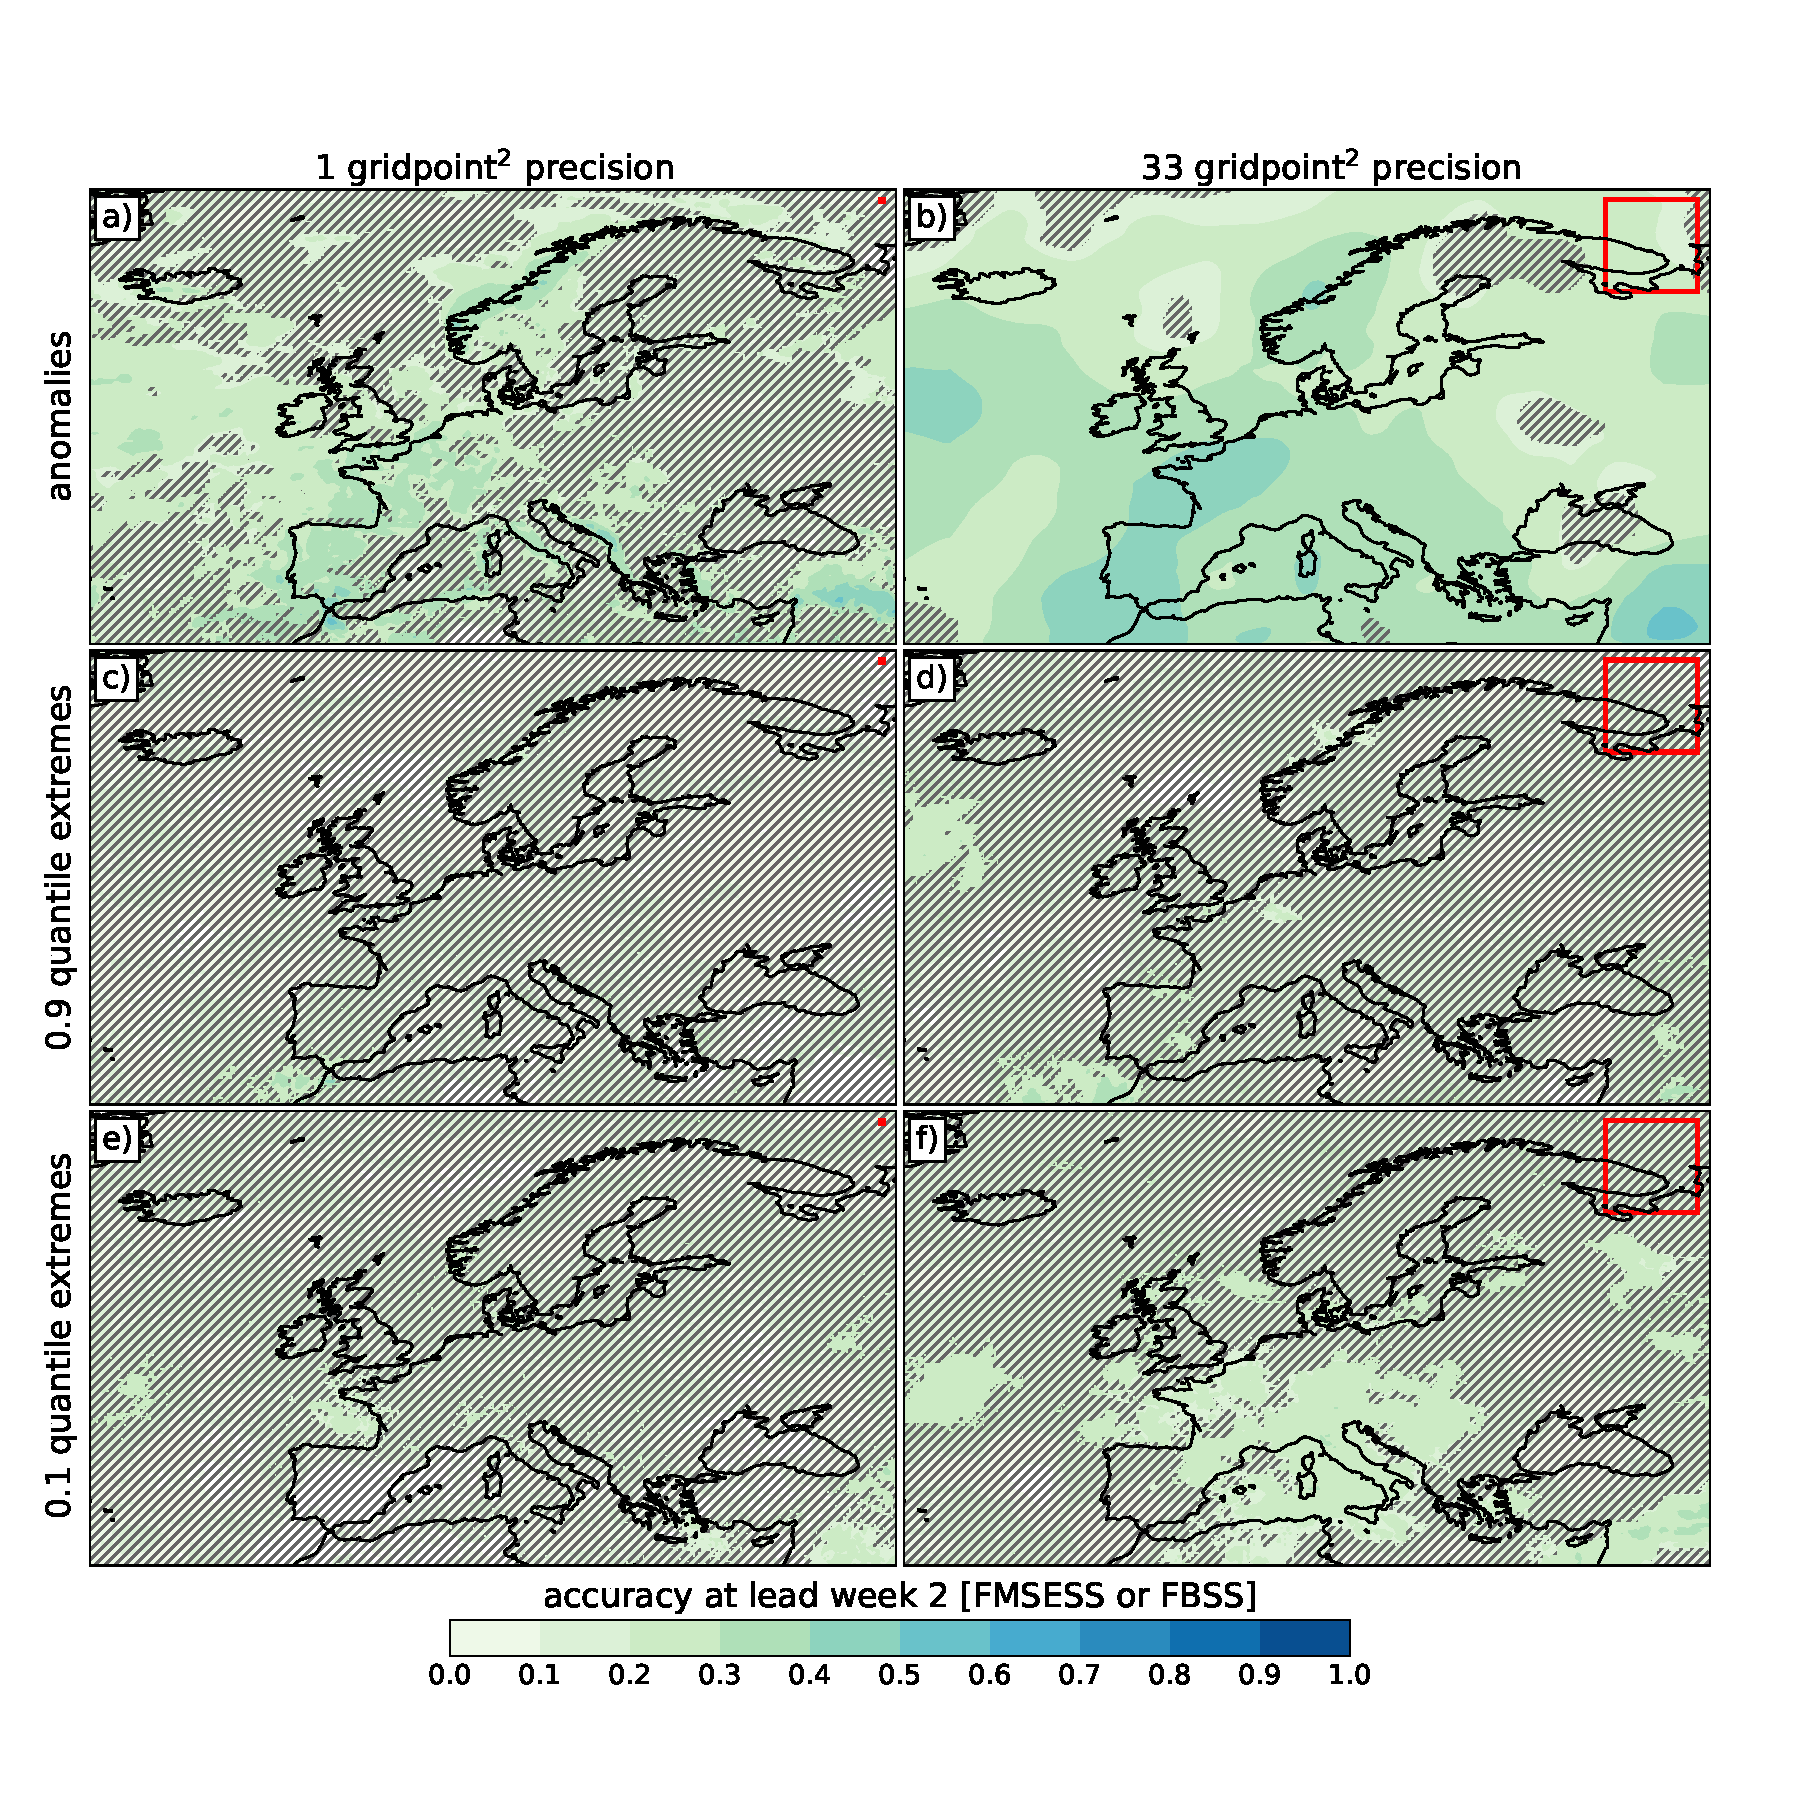
\includegraphics[scale=0.45]{fig_04.png}\\
  \caption{As in Fig.~2 except for weekly-accumulated precipitation forecasts at lead-week 2.}\label{f4}
\end{figure}

\newpage
\begin{figure}[t]
  \noindent\includegraphics[scale=0.7]{fig_05.png}\\
  \caption{As in Fig. 1a except for the Fractions Mean-Square Error Skill Score (FMSESS) over the Scandinavian domain shown in Fig.~6. Black, blue and red arrows denote the use-cases described in section 5.} \label{f5}
\end{figure}

\newpage
\begin{figure}[t]
  \noindent\includegraphics[scale=0.45]{fig_06.png}\\
  \caption{(a-f) Forecasts of storm Hans on August 7$^{th}$ 2023. Shading denotes the ensemble-mean daily-accumulated precipitation for lead days 5 (a,b), 3 (c,d) and 1 (e,f), shown at the grid-scale (left) and with progressively increasing levels of spatial precision (right). Red squares in the upper-right corner of the panels denote the spatial scale of forecast precision. The FMSESS and FBSS for 0.9 quantile extremes are displayed in the top left hand corner of each panel. (g) Daily-accumulated precipitation during Storm Hans on August 7$^{th}$ 2023 according to data from the ERA5 reanalysis. Red stippling denotes Fractions Extreme Forecast Index (FEFI, panels a-f) and Extreme Verification Index (EVI, panel g) values greater than 0.8, signaling an extreme event.} \label{f6}
\end{figure}


%% The Appendices part is started with the command \appendix;
%% appendix sections are then done as normal sections
%\appendix
%\section{Example Appendix Section}
%\label{app1}

%Appendix text.

%% For citations use: 
%%       \citet{<label>} ==> Lamport (1994)
%%       \citep{<label>} ==> (Lamport, 1994)
%%
%Example citation, See \citet{lamport94}.

%% If you have bib database file and want bibtex to generate the
%% bibitems, please use
%%
\bibliographystyle{elsarticle-harv} 
\bibliography{references}

%% else use the following coding to input the bibitems directly in the
%% TeX file.

%% Refer following link for more details about bibliography and citations.
%% https://en.wikibooks.org/wiki/LaTeX/Bibliography_Management

%%\begin{thebibliography}{00}

%% For authoryear reference style
%% \bibitem[Author(year)]{label}
%% Text of bibliographic item

%%\bibitem[Lamport(1994)]{lamport94}
%%  Leslie Lamport,
%%  \textit{\LaTeX: a document preparation system},
%%  Addison Wesley, Massachusetts,
%%  2nd edition,
%%  1994.


%%\end{thebibliography}
\end{document}

\endinput
%%
%% End of file `elsarticle-template-harv.tex'.


